%% LaTeX-Beamer template for KIT design
%% by Erik Burger, Christian Hammer
%% title picture by Klaus Krogmann
%%
%% version 2.1
%%
%% mostly compatible to KIT corporate design v2.0
%% http://intranet.kit.edu/gestaltungsrichtlinien.php
%%
%% Problems, bugs and comments to
%% burger@kit.edu

\documentclass[18pt]{beamer}

%% SLIDE FORMAT

% use 'beamerthemekit' for standard 4:3 ratio
% for widescreen slides (16:9), use 'beamerthemekitwide'

\usepackage{templates/beamerthemekit}
% \usepackage{templates/beamerthemekitwide}

\usepackage[utf8]{inputenc}
\usepackage{hyperref}
\usepackage{listings}

%% TITLE PICTURE

% if a custom picture is to be used on the title page, copy it into the 'logos'
% directory, in the line below, replace 'mypicture' with the
% filename (without extension) and uncomment the following line
% (picture proportions: 63 : 20 for standard, 169 : 40 for wide
% *.eps format if you use latex+dvips+ps2pdf,
% *.jpg/*.png/*.pdf if you use pdflatex)

\titleimage{greendrop}

%% TITLE LOGO

% for a custom logo on the front page, copy your file into the 'logos'
% directory, insert the filename in the line below and uncomment it

%\titlelogo{mylogo}

% (*.eps format if you use latex+dvips+ps2pdf,
% *.jpg/*.png/*.pdf if you use pdflatex)

%% TikZ INTEGRATION

% use these packages for PCM symbols and UML classes
% \usepackage{templates/tikzkit}
% \usepackage{templates/tikzuml}

% the presentation starts here

\title[Konstruktoren und Methoden]{Programmieren:\\ Konstruktoren und Methoden}
\subtitle{Tutorium 30}
\author{YouniS Bensalah}
\date{November 13, 2015}

\institute{Chair for Software Design and Quality}

% Bibliography

\usepackage[citestyle=authoryear,bibstyle=numeric,hyperref,backend=biber]{biblatex}
\addbibresource{templates/example.bib}
\bibhang1em

\begin{document}

% change the following line to "ngerman" for German style date and logos
\selectlanguage{english}

%title page
\begin{frame}
\titlepage
\end{frame}

%table of contents
\begin{frame}{Heute}
\tableofcontents
\end{frame}

\section{Organisatorisches}

\begin{frame}{Immer noch freie Termine in Do-Tutorien}
    Es gibt \textbf{immer noch} noch freie Plätze (ca. 14) in folgenden Tutorien:
    \begin{itemize}
        \item Do 11:30 - 13:00, 50.34 Raum -120 (Peter Oettig)
        \item Do 11:30 - 13:00, 50.34 Raum -119 (Florian Heller)
    \end{itemize}
    Die Studenten, die ihr Tutorium wechseln möchten, können eine E-Mail an folgende Adresse schicken:\\
    \begin{center}
    {\Large programmieren-vorlesung@ipd.kit.edu}
    \end{center}
\end{frame}

\begin{frame}{In manchen Tutorien gerade...}
    \begin{figure}
        
\includegraphics[scale=.5]{img/tuturien.jpg}
    \end{figure}
\end{frame}


\section{Konstruktoren}

\begin{frame}{Konstruktoren}
    \begin{itemize}
        \item Der \textbf{Konstruktor} ist eine spezielle Methode, die beim Erstellen eines neuen Objekts (\texttt{new}) aufgerufen wird.
        \item Attribute werden initialisiert.
        \item Das neue Objekt erhält einen gültigen Startzustand.
    \end{itemize}
\end{frame}

\begin{frame}{Default-Konstruktor}
    \begin{itemize}
        \item Java stellt für jede Klasse zunächst einen \textbf{Default-Konstruktor} (default constructor) zur Verfügung.
        \item Keine Argumente
        \item Alle Attribute werden mit Null* initialisiert.
    \end{itemize}


    \vspace{.5in}
    [*] \textit{Default Values:} \url{https://docs.oracle.com/javase/tutorial/java/nutsandbolts/datatypes.html}

\end{frame}

\begin{frame}[fragile]{Default-Konstruktor}
    \begin{exampleblock}{Beispiel}
        \begin{lstlisting}[language=Java]
public class Dog {}

Dog odie = new Dog();
        \end{lstlisting}

    \end{exampleblock}

\end{frame}

\begin{frame}[fragile]{Default-Konstruktor}
    \begin{exampleblock}{Noch ein Beispiel}
        \begin{lstlisting}[language=Java,basicstyle=\scriptsize]
public class Product {

    private double price;
    private int quantity;
    private String identifier;
    private boolean primeEligible;

    public void display() {
        System.out.println("Price: " + this.price);
        System.out.println("Quantity: " + this.quantity);
        System.out.println("Identifier: " + this.identifier);
        System.out.println("Prime eligible: " + this.primeEligible);
    }

}
        \end{lstlisting}

    \end{exampleblock}

\end{frame}

\begin{frame}[fragile]{Default-Konstruktor}
\begin{exampleblock}{}
    \begin{lstlisting}[language=Java]
Product p = new Product();
p.display();
    \end{lstlisting}
\end{exampleblock}

    \begin{exampleblock}{Ausgabe}
        \begin{lstlisting}
Price: 0.0
Quantity: 0
Identifier: null
Prime eligible: false
        \end{lstlisting}

    \end{exampleblock}

\end{frame}

\begin{frame}{Eigener Konstruktor}
    Es ist möglich, einen eigenen Konstruktor zu definieren.
    \begin{itemize}
        \item Man kann selbst bestimmen, mit welchen Werten das Objekt initialisiert wird.
        \item Welche Werte machen für eine bestimmte Klasse Sinn ?
        \item Anfangswerte können als Parameter übergeben werden.
        \item Prüfen, ob übergebene Werte gültig sind.
    \end{itemize}
\end{frame}

\begin{frame}{Eigener Konstruktor}
    \textit{Der Default-Konstruktor klingt doch praktisch !\\ Brauche ich überhaupt mehr ?}
\end{frame}

\begin{frame}[fragile]{Eigener Konstruktor}
    \begin{exampleblock}{Macht das Sinn ?}
        \begin{lstlisting}[language=Java,basicstyle=\scriptsize]
public class Fraction {

    private int numerator;
    private int denominator;

    public int approximate() {
        return this.numerator / this.denominator;
    }

    // ...

}

Fraction f = new Fraction();
int x = f.approximate();
        \end{lstlisting}

    \end{exampleblock}
\end{frame}

\begin{frame}{Eigener Konstruktor}
    \begin{figure}
        
\includegraphics[scale=0.32]{img/iaccidentallyby0.jpg}
    \end{figure}
\end{frame}

\begin{frame}{Eigener Konstruktor}
    \textbf{Java kann nicht die Bedeutung der Attribute ahnen !}\\
    \vspace{.5in}
    \pause
    Der Entwickler muss also dafür sorgen, dass \dots
    \begin{itemize}
        \item Attribute mit gültigen Werten initialisiert werden (siehe Konstruktor)
        \item Attribute im Laufe der Anwendung keine unzulässigen Werte annehmen
        \item keine Inkonsistenzen auftreten können
        \item ein Objekt nicht in einen ungültigen Zustand geraten kann
    \end{itemize}
\end{frame}

\begin{frame}[fragile]{Eigener Konstruktor}
    Man definiert einen Konstruktor in Java wie folgt:
    \begin{exampleblock}{Konstruktor}
        \begin{lstlisting}[language=Java]
public class Dog {

    public Dog(...) {
        ...
    }

}
        \end{lstlisting}

    \end{exampleblock}

\end{frame}

\begin{frame}{Eigener Konstruktor}
    \textit{\dots also wie eine Methode ?} - \textbf{Fast !}
    \begin{itemize}
        \item Kein Rückgabetyp
        \item Auch nicht \texttt{void}
        \item Methodenname == Klassenname
    \end{itemize}
\end{frame}

\begin{frame}[fragile]{Eigener Konstruktor}
    \begin{exampleblock}{Beispiel 1}
        \begin{lstlisting}[language=Java]
public class Cat {

    private int lives;

    public Cat() {
        this.lives = 9;
    }

}
        \end{lstlisting}

    \end{exampleblock}

\end{frame}

\begin{frame}[fragile]{Eigener Konstruktor}
    \begin{exampleblock}{Beispiel 2}
        \begin{lstlisting}[language=Java]
public class Dog {

    private String name;

    public Dog(String name) {
        this.name = name;
    }

}
        \end{lstlisting}

    \end{exampleblock}

\end{frame}


\begin{frame}[fragile]{Eigener Konstruktor}
    \textit{\dots aber wie rufe ich den Konstruktor auf ?}
    \pause
    \\
    \vspace{.2in}
    {\huge Mit \texttt{new} !}
    \vspace{.2in}
    \begin{exampleblock}{Konstruktor}
        \begin{lstlisting}[language=Java]
Cat garfield = new Cat();
Dog odie = new Dog("Odie");
        \end{lstlisting}

    \end{exampleblock}
\end{frame}


\begin{frame}{Eigener Konstruktor}
    \begin{alertblock}{Vorsicht !}
        Sobald man einen eigenen Konstruktor definiert, \textbf{verschwindet der Default-Konstruktor} von Java.
    \end{alertblock}
\end{frame}

\begin{frame}[fragile]{Eigener Konstruktor}
    \begin{exampleblock}{Das wäre auch zu schön}
        \begin{lstlisting}[language=Java]
public class Dog {

    private String name;

    public Dog(String name) {
        this.name = name;
    }

}

Dog struppi = new Dog("Struppi");  // ok
Dog odie = new Dog();  // nicht mehr ok
        \end{lstlisting}

    \end{exampleblock}


\end{frame}

\begin{frame}[fragile]{Eigener Konstruktor}
    \begin{exampleblock}{Jetzt geht es wieder}
        \begin{lstlisting}[language=Java,basicstyle=\scriptsize]
public class Dog {
    // ...

    public Dog() {
        this.name = "Odie";
    }

    public Dog(String name) {
        this.name = name;
    }

}

Dog struppi = new Dog("Struppi");  // ok
Dog odie = new Dog();  // jetzt auch ok
        \end{lstlisting}

    \end{exampleblock}

    \pause
    \textit{Hä \dots wie geht das ?}
    \pause
    \textbf{- Kommt gleich !}

\end{frame}


\begin{frame}{this-Referenz}
    Die \texttt{this}-Referenz erlaubt es, innerhalb einer Methode auf Attribute des Objekts zuzugreifen.
    \begin{itemize}
        \item Unterscheidung zwischen \textbf{Attributen} und \textbf{Variablen}
        \item \texttt{this} ist vordefiniert !
    \end{itemize}
\end{frame}

\begin{frame}[fragile]{this-Referenz}
    \begin{exampleblock}{Beispiel}
        \begin{lstlisting}[language=Java]
public class Dog {

    private String name;

    public Dog(String name) {
        this.name = name;
    }

    public void sayName() {
        System.out.println("Wauwau wau " + this.name);
    }

}
        \end{lstlisting}

    \end{exampleblock}

\end{frame}

\begin{frame}[fragile]{this-Referenz}
    \begin{exampleblock}{}
        \begin{lstlisting}[language=Java]
Dog odie = new Dog("Odie");
Dog struppi = new Dog("Struppi");

odie.sayName();
struppi.sayName();
        \end{lstlisting}

    \end{exampleblock}

    \begin{exampleblock}{Ausgabe}
        \begin{lstlisting}[language=Java]
Wauwau wau Odie
Wauwau wau Struppi
        \end{lstlisting}

    \end{exampleblock}

\end{frame}

\begin{frame}{Mehrere Konstruktoren}
    Java erlaubt es, \textit{mehrere} Konstruktoren zu definieren.
    \begin{itemize}
        \item Die Konstruktoren müssen sich in Anzahl oder Typ ihrer Argumente unterscheiden
        \item Erzeugen eines Objekts auf verschiedene Weise möglich
    \end{itemize}
\end{frame}

\begin{frame}[fragile]{Mehrere Konstruktoren}
    \begin{exampleblock}{Beispiel}
        \begin{lstlisting}[language=Java,basicstyle=\scriptsize]
public class Color {

    public Color(int red, int green, int blue) { ... }

    public Color(int red, int green, int blue, int alpha) { ... }

    public Color(String hex) { ... }

    public Color() { ... }

}
        \end{lstlisting}

    \end{exampleblock}

\end{frame}

\begin{frame}[fragile]{Mehrere Konstruktoren}
    \begin{exampleblock}{Beispiel}
        \begin{lstlisting}[language=Java]
Color lime, pink, lightblue, black;

lime            = new Color(180, 255, 32);
pink            = new Color(255, 56, 246, 180);
lightblue       = new Color("4ABAFF");
black           = new Color();

        \end{lstlisting}

    \end{exampleblock}
\end{frame}


\section{Methoden}

\begin{frame}[fragile]{Methoden}
    Methoden \dots
    \begin{itemize}
        \item beschreiben das Verhalten von Objekten
        \item können Berechnungen durchführen
        \item können Werte züruckgeben
        \item können den Zustand des Objekts verändern
    \end{itemize}



\end{frame}

\begin{frame}[fragile]{Parameter}
    \begin{itemize}
        \item Ein Parameter ist eine spezielle Variable, welche einen an eine Methode übergebenen Wert beinhaltet.
        \pause
        \item Es wird zwischen \textbf{formalen} und \textbf{aktuellen} Parametern unterschieden:
        \begin{itemize}
            \item Formaler Parameter: Der Name, der bei der Deklaration der Methode gewählt wurde
            \item Aktueller Parameter: Der Wert, der beim Aufruf für den formalen Parameter eingesetzt wird
        \end{itemize}
    \end{itemize}

    \pause
    \begin{exampleblock}{Beispiel}
        \begin{lstlisting}[language=Java]
public Dog(String name) { ... } // formaler parameter

String someName = "Odie";
Dog odie = new Dog(someName);  // aktueller parameter
        \end{lstlisting}
    \end{exampleblock}

\end{frame}

\begin{frame}{Lokale Variablen}
    \textbf{Lokale Variablen}
    \begin{itemize}
        \item sind Hilfsspeicher für Zwischengrößen in Methoden
        \item werden auf dem \textbf{Stack} abgelegt
        \item existieren nur, solange die Methode abgearbeitet wird
        \item \alert{werden nicht automatisch initialisiert}
    \end{itemize}
\end{frame}

\begin{frame}[fragile]{Lokale Variablen}
    \begin{exampleblock}{Beispiel}
        \begin{lstlisting}[language=Java]
public void swapCoordinates() {
    int temp = this.x;  // lokale hilfsvariable
    this.x = this.y;
    this.y = temp;
}
        \end{lstlisting}
    \end{exampleblock}

\end{frame}

\begin{frame}[fragile]{void}
    Der Rückgabetyp \texttt{void} wird verwendet, wenn eine Methode \textbf{keinen Wert zurückgeben} soll.

    \begin{exampleblock}{Beispiel}
        \begin{lstlisting}[language=Java]
public void setXCoordinate(int x) {
    this.xCoordinate = x;
}
        \end{lstlisting}
    \end{exampleblock}



\end{frame}

\begin{frame}{Wert - Referenz}
    body
\end{frame}

\begin{frame}{Private Methoden}
    body
\end{frame}

\begin{frame}{Überladen von Methoden}
    body
\end{frame}

\begin{frame}{Statische Methoden}
    body
\end{frame}

\begin{frame}[fragile]{Main}
    Die \texttt{main}-Methode:
    \begin{itemize}
        \item ist eine statische Methode
        \item markiert den Startpunkt des Programms
    \end{itemize}

    \begin{exampleblock}{\texttt{main}}
        \begin{lstlisting}[language=Java]
public static void main(String argv[]) {
    // do something...
}
        \end{lstlisting}

    \end{exampleblock}


\end{frame}

\begin{frame}[fragile]{argv[]}
    \texttt{argv[]} enthält die Parameter, welche in der Kommandozeile an das Programm übergeben werden.
    \pause
    \begin{exampleblock}{Kommandozeile}
        \begin{lstlisting}
% java MyProgram 42 -v 9000 foo
        \end{lstlisting}
    \end{exampleblock}

\end{frame}

\begin{frame}[fragile]{argv[]}

    \begin{exampleblock}{Im Programm}
        \begin{lstlisting}[language=Java]
public class MyProgram {

    public static void main(String argv[]) {
        System.out.println("argv[0] ist " + argv[0]);
        System.out.println("argv[1] ist " + argv[1]);
        System.out.println("argv[2] ist " + argv[2]);
        System.out.println("argv[3] ist " + argv[3]);
    }

}
        \end{lstlisting}
    \end{exampleblock}

\end{frame}

\begin{frame}[fragile]{argv[]}

    \begin{exampleblock}{Ausgabe}
        \begin{lstlisting}
argv[0] ist 42
argv[1] ist -v
argv[2] ist 9000
argv[3] ist foo
        \end{lstlisting}
    \end{exampleblock}

\end{frame}


\begin{frame}{Statische Attribute}
    body
\end{frame}

\begin{frame}{Standard Ein- und Ausgabe}
    body
\end{frame}

\appendix
\beginbackup

\begin{frame}{Fragen ?}
    \begin{figure}
        
\includegraphics[scale=0.3]{img/fragen.jpg}
    \end{figure}
\end{frame}

\begin{frame}{Bis nächste Woche !}
    \begin{figure}
        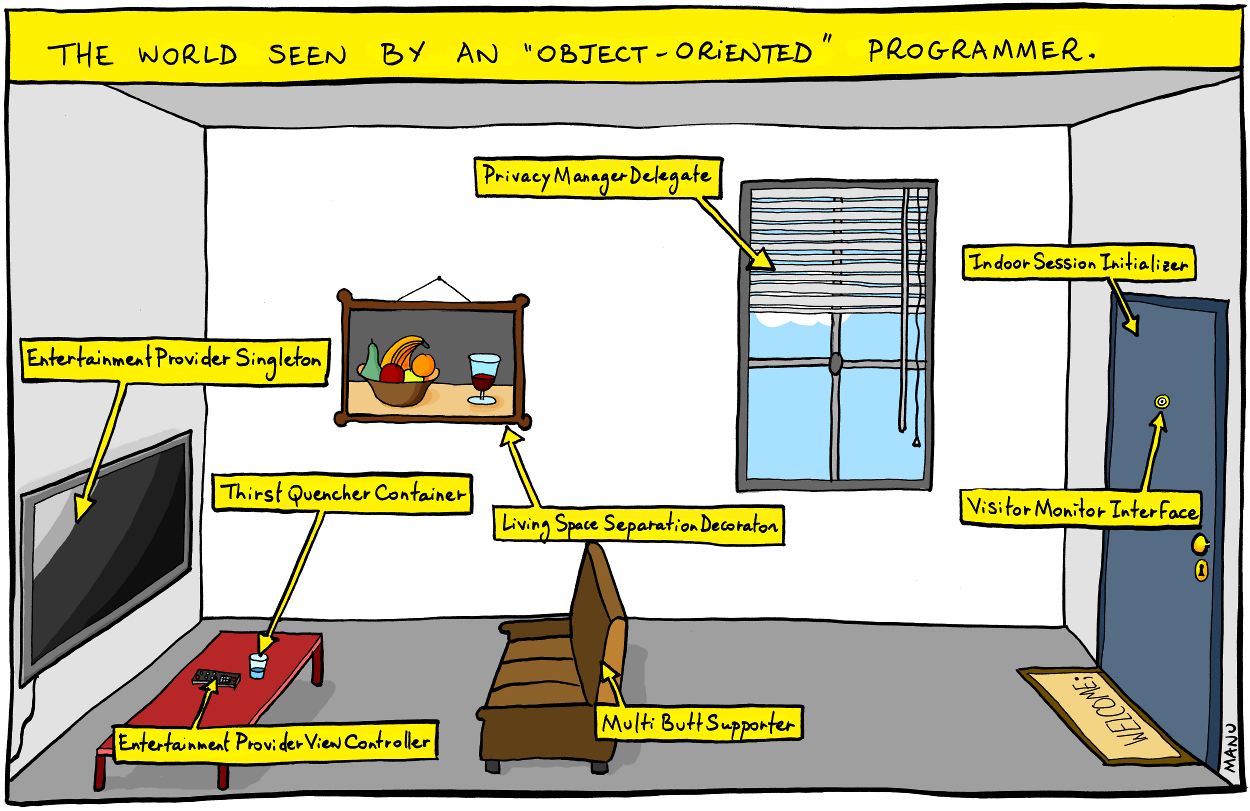
\includegraphics[scale=2]{img/oop.png}
    \end{figure}
\end{frame}

\backupend

\end{document}
